\chapter{Methodology}
\label{sec:methodology}

\begin{German}
    In diesem Kapitel wird das methodische Vorgehen dieser Arbeit beschrieben.
    
    \begin{quote}
        Without a framework that is shared by authors, reviewers, and editors, DS research runs the danger of being mistaken for poor-quality empirical research or for practice case study“ \textcite{peffersPDFDesignScience2024}.\\
    \end{quote}
    
    Um dies zu vermeiden, wird in dieser Arbeit die wissenschaftlich fundierte Design Science Research Methodology (DSRM) von Peffers et al. \cite{peffersPDFDesignScience2024} herangezogen. Diese Methodologie stellt einen strukturierten Rahmen bereit, um innovative Artefakte systematisch zu entwickeln und gleichzeitig wissenschaftliche Erkenntnisse zu generieren. Die DSRM umfasst sechs Schritte, die bei Bedarf iterativ durchlaufen werden können (vgl. \ref{fig:DSR}).
\end{German}

\begin{English}
    In this chapter, the methodological approach of this work is described. It explains how the Scan-to-BIM framework was developed and which steps were followed in the process.

    \begin{quote}
        Without a framework that is shared by authors, reviewers, and editors, DS research runs the danger of being mistaken for poor-quality empirical research or for practice case study - \textcite{peffersPDFDesignScience2024}.\\
    \end{quote}
    
    To avoid this, the scientifically grounded Design Science Research Methodology (DSRM) by Peffers et al. \cite{peffersPDFDesignScience2024} is used in this work. This methodology provides a structured framework for systematically developing innovative artifacts while generating scientific insights. The DSRM consists of six steps that can be iteratively traversed if necessary (see Figure \ref{fig:DSR}).
\end{English}

\begin{figure}[h]
    \centering
    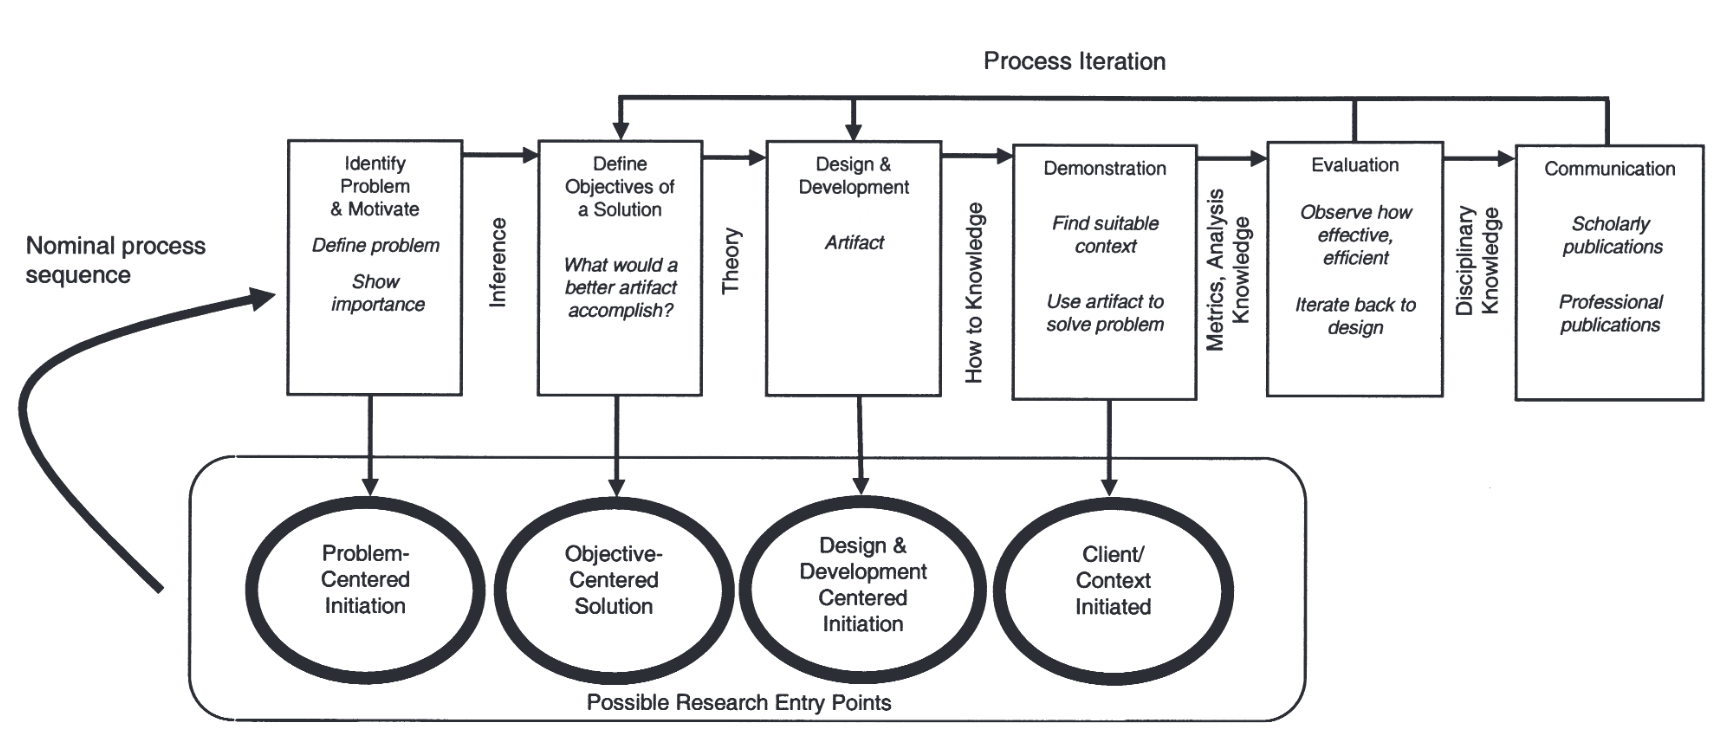
\includegraphics[width=1\textwidth]{images/DSR.png}
    \caption{Design Science Research Methodology (DSRM) \cite{peffersPDFDesignScience2024}}
    \label{fig:DSR}
\end{figure}

\begin{German}
    Die Umsetzung der sechs Schritte erfolgt innerhalb der klassischen Struktur einer weissenschaftlichen Arbeit. 
    Als Artefakt wird in diesem Kapitel auf Basis der Literaturanalyse ein Scan-to-BIM-Framework entwickelt. Dieses zeigt auf taktischer Ebene auf, wie ein automatisierter Scan-to-BIM-Workflow aussehen könnte. 
    Im nächsten Kapitel wird dann auf Basis des Frameworks eine Scan-to-BIM-Pipeline entwickelt. Diese zeigt auf operativer Ebene, dass damit ein automatisierter Scan-to-BIM-Workflow möglich ist.
    In den darauffolgenden Kapiteln wird das Framework anschliessend evaluiert.\\
    Die nachfolgende Tabelle \ref{tab:DSRM_steps} zeigt die Zuordnung der DSRM-Schritte zu den Kapiteln dieser Arbeit.
\end{German}

\begin{English}
    The implementation of the six steps is carried out within the classic structure of a scientific work. 
    As an artifact, this chapter develops a Scan-to-BIM framework based on the literature analysis. This framework illustrates at a tactical level how an automated Scan-to-BIM workflow could look like. 
    In the next chapter, a Scan-to-BIM pipeline is developed based on the framework. This shows at an operational level that an automated Scan-to-BIM workflow is possible.
    In the following chapters, the framework is then evaluated.\\
    The following table \ref{tab:DSRM_steps} shows the mapping of the DSRM steps to the chapters of this work.
\end{English}

\begin{table}[htbp]
    \centering
    \begin{tabular}{ll}
    \toprule
    \textbf{DSRM Step} & \textbf{Thesis Chapter} \\
    \midrule
    1. Problem Identification and Motivation & \ref{sec:research_gap}: \nameref{sec:research_gap} \\
    2. Definition of the Objectives for a Solution & \ref{sec:research_objectives}: \nameref{sec:research_objectives} \\
    3. Design and Development & \ref{sec:design_development}: \nameref{sec:design_development} \\
    4. Demonstration & \ref{sec:case_study}: \nameref{sec:case_study} \\
    5. Evaluation & \ref{sec:results}: \nameref{sec:results} \\
    & \ref{sec:discussion}: \nameref{sec:discussion} \\
    6. Communication & \ref{sec:conclusion}: \nameref{sec:conclusion} \\
    \bottomrule
    \end{tabular}
    \caption{Mapping of DSRM steps to thesis chapters}
    \label{tab:DSRM_steps}
\end{table}
 
\section{Design and Development}
\label{sec:design_development}




\subsection{Data Acquisition}
\begin{German}
Ausgangspunkt des Frameworks ist eine Punktwolke, die Informationen über die gesamte Aussenhülle des zu modellierenden Gebäudes enthält. Sollte das Gebäude Teil einer grösseren Punktwolke sein, ist es zunächst freizustellen.

Aufgrund der hohen Erfassungsgeschwindigkeit und der oft besseren Abdeckung wird der Einsatz einer Drohne für die Datenerfassung empfohlen. Anforderungen an die Qualitätsmetriken der Punktwolke wurden nicht systematisch untersucht. Angesichts der Vorverarbeitungsschritte sowie des ohnehin hohen Generalisierungsgrads bei der geometrischen Rekonstruktion ist jedoch davon auszugehen, dass die meisten Punktwolken, die mit aktuellen Drohnen erfasst werden, den Anforderungen genügen.

Da fehlende Bereiche nicht rekonstruiert werden können, ist die Abdeckung als das zentrale Qualitätskriterium der Punktwolke zu betrachten. Darüber hinaus ist die Richtigkeit wohl relevanter als die Präzision, da Ausreisser im Rahmen der Vorverarbeitung entfernt und Punktlagen geglättet bzw. gemittelt werden. Auf eine besonders hohe Punktdichte kann verzichtet werden, da die Punktanzahl bei durchschnittlich grossen Gebäuden ohnehin reduziert werden muss, um die Konvergenz der geometrischen Rekonstruktion sicherzustellen.
\end{German}

\begin{English}
The starting point of the framework is a point cloud that contains information about the entire outer shell of the building to be modeled. If the building is part of a larger point cloud, it must first be isolated.

Due to the high acquisition speed and often better coverage, the use of a drone for data acquisition is recommended. Requirements for the quality metrics of the point cloud were not systematically investigated. However, given the preprocessing steps and the already high level of generalization in geometric reconstruction, it can be assumed that most point clouds captured with current drones will meet the requirements.

Since missing areas cannot be reconstructed, coverage is to be considered the central quality criterion of the point cloud. In addition, trueness is likely to be more relevant than precision, as outliers are removed during preprocessing and point positions are smoothed or averaged. A particularly high point density can be dispensed with, as the number of points in average-sized buildings must be reduced anyway to ensure the convergence of geometric reconstruction.
\end{English}

\subsection{Preprocessing}
\begin{German}
Zur Vorverarbeitung der Punktwolken wird der Einsatz eines Ausreisserfilters sowie eines Downsamplings empfohlen.

Die Wirksamkeit eines Ausreisserfilters wurde in dieser Arbeit zwar nicht systematisch untersucht, sein Einsatz erscheint jedoch grundsätzlich sinnvoll, da grobe Fehler die Richtigkeit der Rekonstruktion beeinträchtigen können.

Das Downsampling hingegen ist zwingend erforderlich, da die Laufzeit der geometrischen Rekonstruktion überlinear mit der Punktanzahl ansteigt. Bei durchschnittlich grossen Gebäuden kann dies ohne Reduktion der Punktdichte zu Laufzeitüberschreitungen oder Instabilitäten während der Geometrischen Rekonstruktion führen.

Nachfolgend sollen die beiden Vorverarbeitungsschritte im Detail beschrieben werden:\\
\end{German}

\begin{English}
For preprocessing the point clouds, the use of an outlier filter and downsampling is recommended.

The effectiveness of an outlier filter was not systematically investigated in this work, but its use generally seems reasonable, as gross errors can affect the trueness of the reconstruction.

Downsampling, on the other hand, is essential, as the runtime of geometric reconstruction increases superlinearly with the number of points. In average-sized buildings, this can lead to runtime overruns or instabilities during geometric reconstruction without reducing point density.

The two preprocessing steps will be described in detail below:\\
\end{English}

\subsubsection{Statistical Outlier Removal (SOR)}
\begin{German}
    Statistical Outlier Removal entfernt Punkte, die deutlich weiter von ihren Nachbarn entfernt sind als der Durchschnitt.  
    Für jeden Punkt $i = 1, \dots, n$ wird ein lokales Nachbarschaftsmodell mit $k$ nächstgelegenen Punkten berechnet, und die Distanzen $d_{ij}$ zu den Nachbarn $j = 1, \dots, k$ werden bestimmt.

    Die mittlere Distanz $\mu$ und die Standardabweichung $\sigma$ der Punkt-Nachbar-Distanzen ergeben sich aus:

    \[
    \mu = \frac{1}{nk} \sum_{i=1}^{n} \sum_{j=1}^{k} d_{ij}, \quad
    \sigma = \sqrt{ \frac{1}{nk} \sum_{i=1}^{n} \sum_{j=1}^{k} (d_{ij} - \mu)^2 }
    \]

    Ein Punkt wird entfernt, wenn sein durchschnittlicher Nachbarabstand außerhalb eines definierten Bereichs liegt.  
    Zum Beispiel wird ein Punkt $i$ als Ausreisser entfernt, wenn:

    \[
    \bar{d}_i > \mu + \alpha \cdot \sigma
    \]

    wobei $\bar{d}_i$ der mittlere Abstand von Punkt $i$ zu seinen $k$ Nachbarn ist und $\alpha$ ein frei wählbarer Schwellenwert ist (typisch z.B. $\alpha = 1.0\text{-}2.0$). \cite{liu3DPointCloud2021}
\end{German}

\begin{English}
    Statistical Outlier Removal removes points that are significantly further away from their neighbors than the average.  
    For each point $i = 1, \dots, n$, a local neighborhood model is calculated with $k$ nearest points, and the distances $d_{ij}$ to the neighbors $j = 1, \dots, k$ are determined.

    The mean distance $\mu$ and the standard deviation $\sigma$ of the point-neighbor distances are given by:

    \[
    \mu = \frac{1}{nk} \sum_{i=1}^{n} \sum_{j=1}^{k} d_{ij}, \quad
    \sigma = \sqrt{ \frac{1}{nk} \sum_{i=1}^{n} \sum_{j=1}^{k} (d_{ij} - \mu)^2 }
    \]

    A point is removed if its average neighbor distance lies outside a defined range.  
    For example, a point $i$ is removed as an outlier if:

    \[
    \bar{d}_i > \mu + \alpha \cdot \sigma
    \]

    where $\bar{d}_i$ is the average distance of point $i$ to its $k$ neighbors and $\alpha$ is a freely selectable threshold (typically e.g. $\alpha = 1.0\text{-}2.0$). \cite{liu3DPointCloud2021}
\end{English}





\subsubsection{Voxel Grid Downsampling}
\begin{German}
    Voxel Grid Downsampling reduziert die Anzahl von Punkten in einer Punktwolke, indem der Raum in ein regelmässiges 3D-Gitter (Voxelgitter) mit fester Zellgrösse $r$ unterteilt wird. Innerhalb jeder Voxelzelle wird ein repräsentativer Punkt bestimmt (z.\,B. zufällig, Zentrum oder Schwerpunkt), der die übrigen Punkte ersetzt.

    Zunächst werden die minimalen und maximalen Koordinaten bestimmt:

    \[
    x_{\min} = \min(x_1, \dots, x_n), \quad x_{\max} = \max(x_1, \dots, x_n)
    \]

    Analog für $y$ und $z$.

    Jeder Punkt $p_i = (x_i, y_i, z_i)$ wird dann einer Voxelzelle über den diskreten Index

    \[
    i_x = \left\lfloor \frac{x_i - x_{\min}}{r} \right\rfloor, \quad
    i_y = \left\lfloor \frac{y_i - y_{\min}}{r} \right\rfloor, \quad
    i_z = \left\lfloor \frac{z_i - z_{\min}}{r} \right\rfloor
    \]

    zugewiesen. Pro Zelle wird genau ein Punkt übernommen, um die Punktwolke zu approximieren.
\end{German}

\begin{English}
    Voxel Grid Downsampling reduces the number of points in a point cloud by dividing the space into a regular 3D grid (voxel grid) with a fixed cell size $r$. Within each voxel cell, a representative point is determined (e.g., randomly, center, or centroid), which replaces the remaining points.

    First, the minimum and maximum coordinates are determined:

    \[
    x_{\min} = \min(x_1, \dots, x_n), \quad x_{\max} = \max(x_1, \dots, x_n)
    \]

    Similarly for $y$ and $z$.

    Each point $p_i = (x_i, y_i, z_i)$ is then assigned to a voxel cell using the discrete index

    \[
    i_x = \left\lfloor \frac{x_i - x_{\min}}{r} \right\rfloor, \quad
    i_y = \left\lfloor \frac{y_i - y_{\min}}{r} \right\rfloor, \quad
    i_z = \left\lfloor \frac{z_i - z_{\min}}{r} \right\rfloor
    \]

    Exactly one point is retained per cell to approximate the point cloud. \cite{liu3DPointCloud2021}
\end{English}

\subsection{Geometric Reconstruction}
\begin{German}
    Für die geometrische Rekonstruktion wird das Framework \textit{PolyFit} von Nan et al. \cite{nanPolyFitFramework2023} vergeschlagen. Es extrahiert aus einer Punktwolke zusammenhängende, planare Flächenbereiche und rekonstruiert diese als trianguliertes, aber global planares Mesh. Das Mesh ist manifold (topologisch korrekt) und wasserdicht, d.h. es hat keine Löcher und keine überlappenden Flächen. Das Framework ist auf die Rekonstruktion von ebenen Flächen fokussiert, was es für die meisten Anwendungsfälle im Bauwesen geeignet macht, da die meisten Bauteile wie Wände, Decken und Böden eben sind. Für gekrümmte Geometrien ist das Framework hingegen nicht geeignet. Es ist zudem zu beachten, dass nicht die Bauteile selbst modelliert werden, sondern lediglich die durch ihre Oberflächen aufgespannten Hüllen.
    
    Das Framework wurde in C++ implementiert und ist auf GitHub öffentlich zugänglich \cite{nanLiangliangNanPolyFit2025}. Zunächst werden mit dem RANSAC-Algorithmus (Random Sample Consensus) Ebenen in der Punktwolke identifiziert. Ähnliche Ebenen werden zusammengeführt, um robuste Flächen zu erhalten. Durch paarweise Schnittmengen der Ebenen entstehen Polygonflächen. Durch binäre lineare Optimierung wird aus einer Menge von Kandidatenflächen $F = \{f_1, f_2, \dots, f_N\}$ eine Teilmenge ausgewählt, die die Punktwolke möglichst gut beschreibt und gleichzeitig ein kompaktes, topologisch korrektes Modell bildet.

    \vspace{1em}
    \noindent
    \textbf{Zielfunktion:}
    \[
    \min_{\mathbf{x}} \quad
    \lambda_f \cdot E_f + \lambda_m \cdot E_m + \lambda_c \cdot E_c
    \]

    \vspace{1em}
    \noindent
    \textbf{Erläuterung:}
    \begin{itemize}
    \item $\mathbf{x} = (x_1, \dots, x_N)$ ist ein Vektor binärer Entscheidungsvariablen:
        \[
        x_i =
        \begin{cases}
        1, & \text{wenn Fläche } f_i \text{ ausgewählt wird} \\
        0, & \text{sonst}
        \end{cases}
        \]
    \item $E_f$: \textit{Datenanpassung} - bevorzugt Flächen, die gut zur Punktwolke passen.
    \item $E_m$: \textit{Modellkomplexität} - bestraft scharfe Kanten und kleine Details.
    \item $E_c$: \textit{Punktabdeckung} - bevorzugt Flächen, die möglichst viele Punkte abdecken.
    \item $\lambda_f$, $\lambda_m$, $\lambda_c$: Gewichtungsfaktoren zur Steuerung der Einflussgrössen.
    \end{itemize}

    \vspace{1em}
    \noindent
    \textbf{Nebenbedingungen:}
    \[
    \sum_{j \in \mathcal{N}(e_i)} x_j \in \{0, 2\} \quad \forall e_i \in E
    \]
    \begin{itemize}
    \item Jede Kante $e_i$ muss entweder gar nicht oder genau von zwei Flächen genutzt werden, um ein \textit{manifold} und \textit{wasserdichtes} Modell sicherzustellen.
    \end{itemize}

    \[
    x_i \in \{0, 1\} \quad \forall i = 1, \dots, N
    \]
    \begin{itemize}
    \item Binäre Entscheidung: Fläche wird aufgenommen oder verworfen.
    \end{itemize}

\end{German}

\begin{English}
    For geometric reconstruction, the framework \textit{PolyFit} by Nan et al. \cite{nanPolyFitFramework2023} is proposed. It extracts connected planar surface regions from a point cloud and reconstructs them as a triangulated but globally planar mesh. The mesh is manifold (topologically correct) and watertight, meaning it has no holes and no overlapping surfaces. The framework focuses on reconstructing flat surfaces, making it suitable for most applications in construction, as most building components like walls, ceilings, and floors are flat. However, it is not suitable for curved geometries. It should also be noted that the components themselves are not modeled, but rather the envelopes defined by their surfaces.

    The framework is implemented in C++ and publicly available on GitHub \cite{nanLiangliangNanPolyFit2025}. Initially, planes in the point cloud are identified using the RANSAC (Random Sample Consensus) algorithm. Similar planes are merged to obtain robust surfaces. Pairwise intersections of the planes create polygonal surfaces. Binary linear optimization selects a subset from a set of candidate surfaces $F = \{f_1, f_2, \dots, f_N\}$ that best describes the point cloud while forming a compact, topologically correct model.

    \vspace{1em}
    \noindent
    \textbf{Objective Function:}
    \[
    \min_{\mathbf{x}} \quad
    \lambda_f \cdot E_f + \lambda_m \cdot E_m + \lambda_c \cdot E_c
    \]

    \vspace{1em}
    \noindent
    \textbf{Explanation:}
    \begin{itemize}
    \item $\mathbf{x} = (x_1, \dots, x_N)$ is a vector of binary decision variables:
        \[
        x_i =
        \begin{cases}
        1, & \text{if surface } f_i \text{ is selected} \\
        0, & \text{otherwise}
        \end{cases}
        \]
    \item $E_f$: \textit{Data Fit} - prefers surfaces that fit well to the point cloud.
    \item $E_m$: \textit{Model Complexity} - penalizes sharp edges and small details.
    \item $E_c$: \textit{Point Coverage} - prefers surfaces that cover as many points as possible.
    \item $\lambda_f$, $\lambda_m$, $\lambda_c$: weighting factors to control the influence of these terms.
    \end{itemize}

    \vspace{1em}
    \noindent
    \textbf{Constraints:}
    \[
    \sum_{j \in \mathcal{N}(e_i)} x_j \in \{0, 2\} \quad \forall e_i \in E
    \]
    \begin{itemize}
    \item Each edge $e_i$ must either not be used at all or be used by exactly two surfaces to ensure a \textit{manifold} and \textit{watertight} model.
    \end{itemize}
    \[
    x_i \in \{0, 1\} \quad \forall i = 1, \dots, N
    \]
    \begin{itemize}
    \item Binary decision: surface is either included or discarded.
    \end{itemize}
\end{English}

\subsection{Semantic Segmentation}
\begin{German}
    Damit das Mesh der geometrischen Rekonstruktion in ein BIM-Modell überführt werden kann, müssen die Flächen zunächst semantisch segmentiert werden. Dies bedeutet, dass die Flächen den entsprechenden Bauteilen zugeordnet werden müssen. Dafür wird ein eigenes, regelbasiertes Segmentationsverfahren angewendet, das auf den Eigenschaften der Flächen basiert. Die Segmentierung erfolgt in zwei Schritten:

    \begin{enumerate}
        \item \textbf{Feature Extraction:} Zunächst wird das Mesh-Modell so ausgerichtet, dass die grösste Fläche in der $x$-$y$-Ebene liegt. Anschliessend wird für jede Fläche des Meshes der zugehörige Normalenvektor berechnet, welcher die räumliche Orientierung der Fläche beschreibt.
        \item \textbf{Classification:} Anschliessend werden die Flächen basierend auf der Ausrichtung ihrer Normalenvektoren in folgende Klassen eingeteilt:
        
        \begin{equation*}
        \text{SurfaceType}(n_i) = 
        \begin{cases}
            \text{Wand}, & \text{wenn } |\hat{z}_i| \approx 0 \\
            \text{Platte}, & \text{wenn } \sqrt{\hat{x}_i^2 + \hat{y}_i^2} \approx 0 \\
            \text{Roof}, & \text{sonst}
        \end{cases}
        \end{equation*}
        wobei $n_i$ der Normalenvektor der Fläche $i$ ist und $\hat{x}_i$, $\hat{y}_i$, $\hat{z}_i$ die normierten Komponenten des Vektors sind. Horizontale Flächen werden zu Platten, vertikale Flächen zu Wänden und geneigte Flächen zu Dächern.
    \end{enumerate}
\end{German}

\begin{English}
    In order to transfer the mesh from the geometric reconstruction into a BIM model, the surfaces must first be semantically segmented. This means that the surfaces need to be assigned to the corresponding building components. A custom rule-based segmentation method is applied, based on the properties of the surfaces. The segmentation is performed in two steps:

    \begin{enumerate}
        \item \textbf{Feature Extraction:} First, the mesh model is oriented so that the largest surface lies in the $x$-$y$ plane. Then, for each surface of the mesh, the associated normal vector is calculated, which describes the spatial orientation of the surface.
        \item \textbf{Classification:} The surfaces are then classified based on the orientation of their normal vectors into the following classes:
        
        \begin{equation*}
        \text{SurfaceType}(n_i) = 
        \begin{cases}
            \text{Wall}, & \text{if } |\hat{z}_i| \approx 0 \\
            \text{Slab}, & \text{if } \sqrt{\hat{x}_i^2 + \hat{y}_i^2} \approx 0 \\
            \text{Roof}, & \text{otherwise}
        \end{cases}
        \end{equation*}
        where $n_i$ is the normal vector of surface $i$ and $\hat{x}_i$, $\hat{y}_i$, $\hat{z}_i$ are the normalized components of the vector. Horizontal surfaces are classified as slabs, vertical surfaces as walls, and inclined surfaces as roofs.
    \end{enumerate}
\end{English}

\subsection{Modeling}
\begin{German}
    Im letzten Schritt wird das semantisch segmentierte Mesh in ein BIM-Modell überführt. Es wird folgender Ansatz empfohlen:
    
    \begin{enumerate}
        \item \textbf{Automatisierte Modellierung:} Für jede Fläche des Meshes wird automatisiert ein entsprechendes Bauteil im BIM-Modell erzeugt. Dabei werden die Geometrie sowie relevante Eigenschaften aus dem Mesh extrahiert und in das BIM-Modell übertragen. Die Zuordnung zu einer Bauteilart (z.B. Wand) erfolgt basierend auf den zuvor definierten Klassen aus der Segmentierung.

        Für eine softwareunabhängige Umsetzung wird empfohlen, die IFC-Schnittstelle zu verwenden. Diese ermöglicht eine standardisierte Übertragung von Geometrie- und Bauteileigenschaften und stellt die Interoperabilität zwischen verschiedenen BIM-Systemen sicher.

        Sollte die nachgelagerte BIM-Software keine vollständige Unterstützung für IFC bieten, kann alternativ die API der jeweiligen Software verwendet werden, um die Bauteile programmgesteuert zu erzeugen. In Fällen, in denen die IFC-Unterstützung eingeschränkt ist, empfiehlt sich die Umwandlung in ein natives Format der Zielsoftware. Dieser Prozess kann beispielsweise durch den Einsatz von visuellen Skriptumgebungen für parametrisches Design automatisiert werden, wie sie in vielen BIM-Plattformen integriert sind. 
        
        Dabei kann jeder Bauteilart (z.B. Wand) ein konkreter Bauteiltyp (z.B. Beton 25 cm) zugewiesen werden. Die native Modellierung ermöglicht eine bessere Integration in die jeweilige Softwareumgebung und erleichtert die spätere Bearbeitung, Analyse und Weiterverwendung der erzeugten Bauteile.

        Am Ende dieses Schrittes sollte ein vollständiges BIM-Modell in LOD 200 vorliegen.

        \item \textbf{Manuelle Modellierung:} Je nach Anwendungsfall kann ein höherer Detaillierungsgrad erforderlich sein. In diesem Fall wird empfohlen, die automatisiert erzeugte Modellierung als Ausgangsbasis zu nutzen und anschliessend manuelle Anpassungen vorzunehmen. Dazu gehört beispielsweise das Ergänzen von Fenstern, Türen oder anderen architektonischen Elementen, die nicht automatisch aus der Punktwolke rekonstruiert werden konnten. Auch die Zuweisung oder Anpassung von Bauteiltypen und -eigenschaften kann in diesem Schritt erfolgen, um den projektspezifischen Anforderungen gerecht zu werden.

        Aus dem so erweiterten Modell lassen sich anschliessend Pläne und Visualisierungen ableiten, die in der weiteren Planung und Ausführung des Bauprojekts verwendet werden können.
    \end{enumerate}
\end{German}

\begin{English}
    In the final step, the semantically segmented mesh is converted into a BIM model. The following approach is recommended:
    
    \begin{enumerate}
        \item \textbf{Automated Modeling:} For each surface of the mesh, a corresponding building component is automatically created in the BIM model. The geometry and relevant properties are extracted from the mesh and transferred to the BIM model. The assignment to a building component type (e.g., wall) is based on the previously defined classes from the segmentation.

        For software-independent implementation, it is recommended to use the IFC interface. This allows for standardized transfer of geometry and building component properties and ensures interoperability between different BIM systems.

        If the downstream BIM software does not fully support IFC, the API of the respective software can be used to programmatically create the components. In cases where IFC support is limited, conversion to a native format of the target software is recommended. This process can be automated using visual scripting environments for parametric design, which are integrated into many BIM platforms.

        Each building component type (e.g., wall) can be assigned a specific building component type (e.g., concrete 25 cm). Native modeling allows for better integration into the respective software environment and facilitates subsequent editing, analysis, and reuse of the generated components.

        At the end of this step, a complete BIM model in LOD 200 should be available.

        \item \textbf{Manual Modeling:} Depending on the application case, a higher level of detail may be required. In this case, it is recommended to use the automatically generated model as a starting point and then make manual adjustments. This includes adding windows, doors, or other architectural elements that could not be automatically reconstructed from the point cloud. The assignment or adjustment of building component types and properties can also take place in this step to meet project-specific requirements.

        From this extended model, plans and visualizations can then be derived for use in further planning and execution of the construction project.
    \end{enumerate}
\end{English}